\documentclass{standalone}
 
\usepackage{tikz}
\usetikzlibrary{automata, positioning}
 \usepackage{color}
\newenvironment{gtext}{\color{gray}}{\ignorespacesafterend}
\newenvironment{btext}{\color{black}}{\ignorespacesafterend}
\definecolor{Set1_5_red}{HTML}{E41A1C}
\definecolor{Set1_5_blue}{HTML}{377EB8}
\begin{document}
    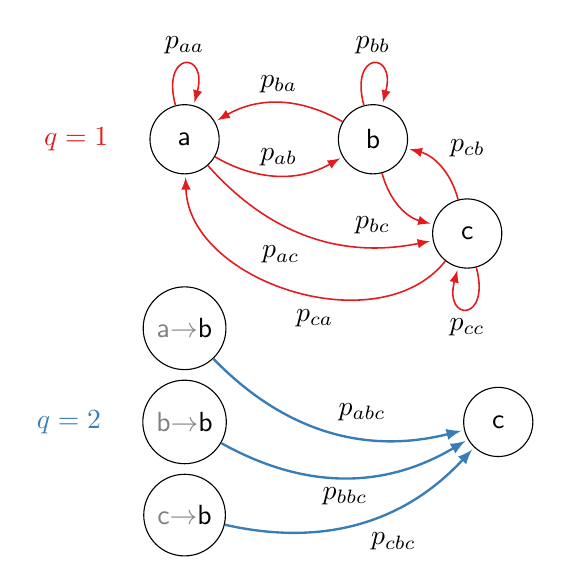
\begin{tikzpicture}[font=\sffamily]
 \begin{scope}[name=q1]
    % Add the states
    \node[state,
          text=black ] (a) {a};
    \node[state,
          right=1.5cm of a,
          text=black] (b) {b};
 \node[state,
          below right= 0.8cm of b,
          text=black] (c) {c};
  \node[left = 0.4cm of a,color=Set1_5_red] {$q=1$};
 
    % Connect the states with arrows
    \draw[every loop,
          auto=right,
          line width=0.2mm,
          >=latex,
          draw=Set1_5_red,
          fill=Set1_5_red]
        (a) edge[bend right, auto=left]  node {$p_{ab}$} (b)
        (b) edge[bend right, auto=right] node {$p_{ba}$} (a)
         (c) edge[bend right, auto=right] node {$p_{cb}$} (b)
         (b) edge[bend right, auto=right] node {$p_{bc}$} (c)
           (c) edge[bend right = -70, auto=left,pos=0.35 ] node {$p_{ca}$} (a)
  (a) edge[bend right, auto=right] node {$p_{ac}$} (c)
        (a) edge[loop above]             node {$p_{aa}$} (a)
        (b) edge[loop above]             node {$p_{bb}$} (b)
        (c) edge[loop below]             node {$p_{cc}$} (c);
\end{scope}

\begin{scope}[yshift = -2.4cm]
    \node[state,
          text=black ] (ab) {\gtext{a$\to$}\btext{b}};
    \node[state,
          below=.12cm of ab,
          text=black] (bb) {\gtext{b$\to$}\btext{b}};
              \node[state,
          right=3cm of bb,
          text=black] (c) {c};
 \node[state,
              below=.12cm of bb,
          text=black] (cb) {\gtext{c$\to$}\btext{b}};
  \node[left = 0.4cm of bb,color=Set1_5_blue] {$q=2$};
  
    \draw[every loop,
          auto=right,
          line width=0.3mm,
          >=latex,
          draw=Set1_5_blue,
          fill=Set1_5_blue]
        (ab) edge[bend right, auto=left]  node {$p_{abc}$} (c)
        (bb) edge[bend right, auto=right] node {$p_{bbc}$} (c)
         (cb) edge[bend right, auto=right] node {$p_{cbc}$} (c);

\end{scope}

   \end{tikzpicture}
\end{document}